


\documentclass[10pt, handout]{beamer}
\setbeamertemplate{navigation symbols}{}
\usefonttheme{serif} 
\usepackage{amsmath}
\usepackage{amssymb}
\usepackage{graphicx}
\usepackage{cite}
\usepackage{color} 
\usepackage{setspace}
\usepackage{hyperref}

\newcommand{\xx}{{\bf{x}}}

\begin{document}
\title{Machine Learning I Lecture VI:\\ Linear models for Classification}   
\author{Jakob H Macke\\ Max Planck Institute for Biological Cybernetics\\ Bernstein Center for Computational Neuroscience} 
\date{XY.XY.2012} 

\frame{\titlepage} 

%\frame{\frametitle{Today: Back to basics of probability theory}} 


\frame{\frametitle{Plan for today}\tableofcontents} 

\section{Binary classification}
\frame{\frametitle{Binary Classification: Assign each data point to one of two classes.} 

%\multicolumn
\begin{columns}
\begin{column}{4cm}
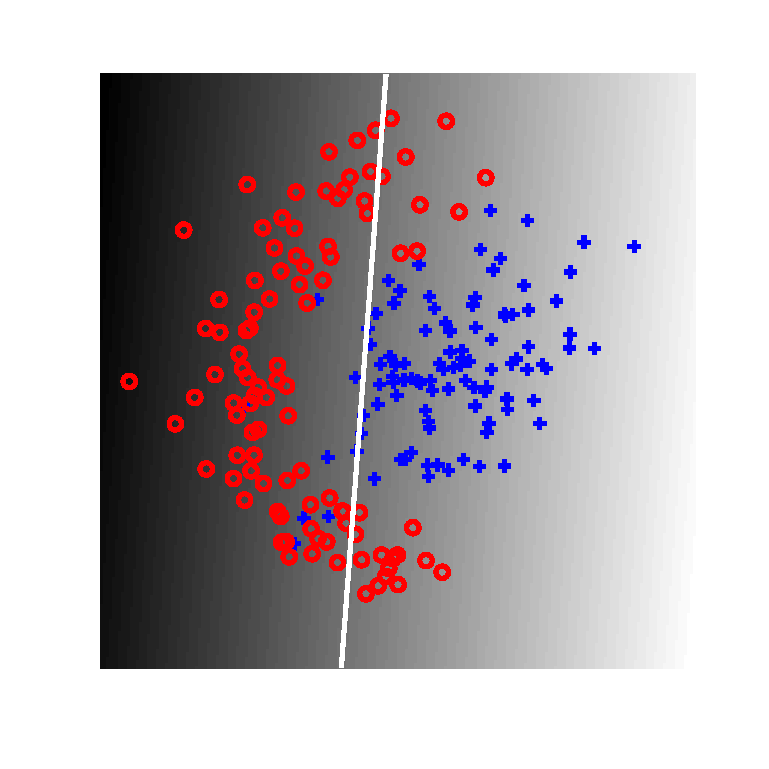
\includegraphics[width=1.1\textwidth]{LinClassification.pdf}
\end{column}
\begin{column}{7.5cm}
Examples:
\begin{itemize}
 \item Is there a face in this image?
\item Will this neuron spike in response to this stimulus?
\item Based on this brain-scan, does this patient have a given disease or not?
\item  Will this customer buy this product or not?
\item Is this person likely to be a democrat/republican? 
\end{itemize}
%\item
 \pause Notation: we have data $D=\{(x_1, t_1),\ldots, (x_N, t_N)\}$, with $t_n=1$ if $x_n$ belongs to class $1$ and $t_n=-1$ if $x_n$ belongs to class $-1$.
\end{column}
\end{columns}
}





\frame{\frametitle{We focus on linear decision rules, also known as `linear discriminant functions'.} 

%\multicolumn

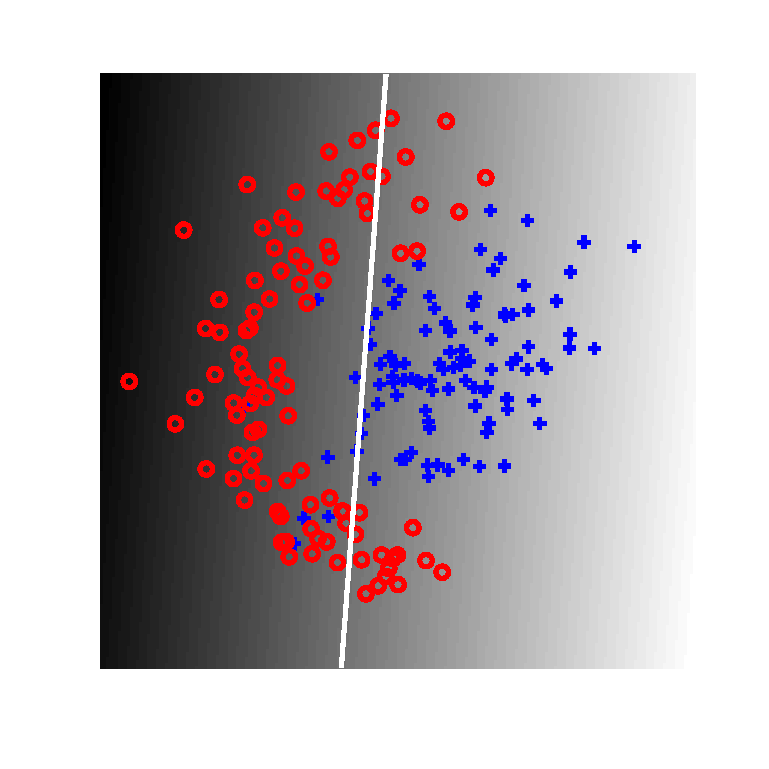
\includegraphics[width=.5\textwidth]{LinClassification.pdf}
\pause
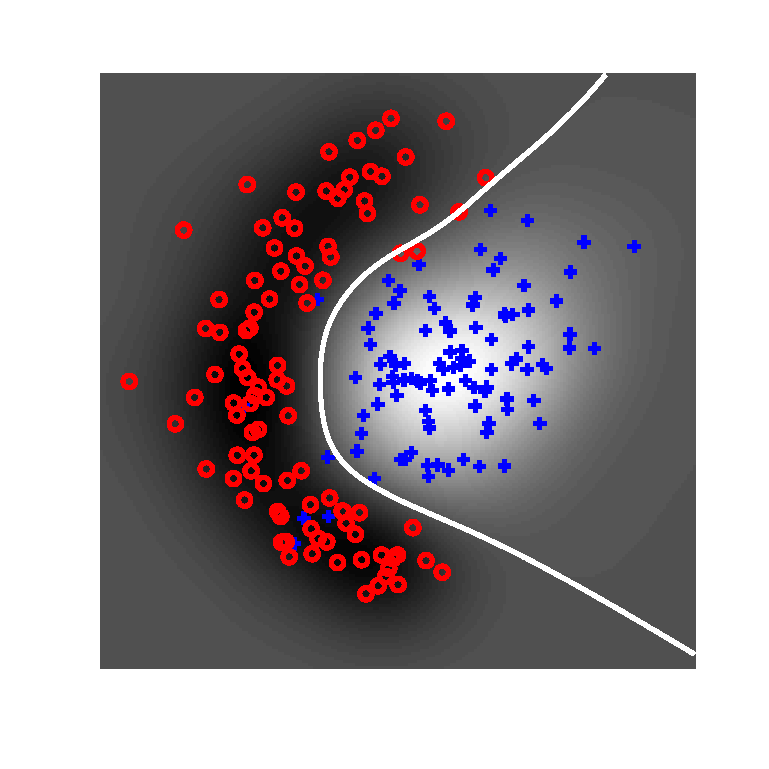
\includegraphics[width=.5\textwidth]{NonLinClassification.pdf}

\pause 

Of course, linear algorithms can be used together with \alert{nonlinear feature spaces} or \alert{nonlinear basis functions} in order to solve nonlinear classification problems!
}

\frame{\frametitle{Linear discriminants separate the space by a hyperplane, and the parameters define its normal vector.} 

%\multicolumn


%\includegraphics[width=.4\textwidth]{LinearSeparators.pdf}
\begin{itemize}
\item Decision function: $y(\xx)=\omega^\top \xx + \omega_o$
\item \pause Classification: \begin{align}
\mbox{if~}y(\xx)>0 & \mbox{~say $\xx$ belongs to class 1}\\
\mbox{if~}y(\xx)<0 & \mbox{~say $\xx$ belongs to class -1}\\
 \end{align}
\item The decision-surface has equation $y(\xx)=0$, and is a hyperplane of dimensionality $D-1$.
\item \pause $\omega$ is the normal vector to the plane, and points into the positive class.
\item \pause $\omega_o$ determines the location of the decision-surface
\item \pause $|y(\xx)|$ is proproptional to the perpendicular distance to the decision-surface (with factor $1$ if $|| \omega ||=1$).
\end{itemize}

}

\frame{\frametitle{Multiple algorithms and methods exist for finding a good $\omega$.} 
\begin{itemize}
\item Mis-classification rate $C(\omega)= \frac{1}{N} \sum_n \delta\left[y(\xx_n) =t_n\right]$ (i.e. average number of errors) difficult to optimize over $\omega$, and might have multiple solutions.
\item \pause Many algorithms can be derived by replacing $C$ by another cost-function which can be optimized.
\item \pause Linear classification algorithms include Least-square classification, Fisher's linear Discriminant, Logistic regression, Support Vector Machines and Rosenblatts' perceptron.
\end{itemize}
}

\section{Least Square Classification}
\frame{\frametitle{You already know one algorithm for linear classification: least square classification.} 
\begin{itemize}
\item We have to fit the function $y(\xx)= \omega^\top \xx+ \omega_o $ to data.
\item \pause Simply do a linear regression from $\xx$ to $t$ by minimizing the sum-of-squared errors $\sum_n (y(\xx_n)-t_n)^2$.
\item \pause $\omega_{reg}=  \left(\sum_n x_n x_n^\top  \right)^{-1} \sum_n x_n t_n$
\item \pause Q: In what situations might this be a bad idea?
\end{itemize}
\pause
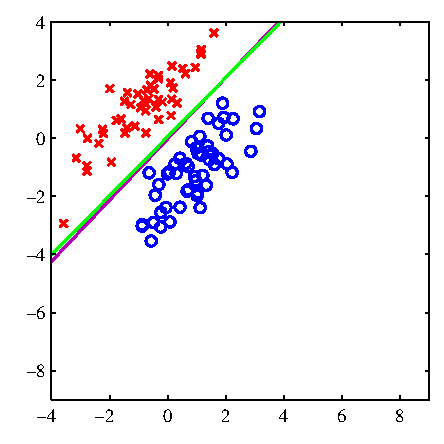
\includegraphics[width=.4\textwidth]{Figure44a.pdf}
\pause
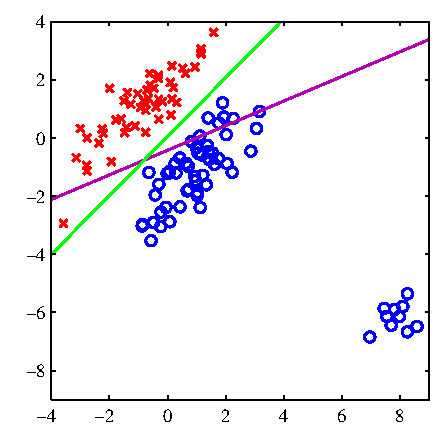
\includegraphics[width=.4\textwidth]{Figure44b.pdf}
\\
\tiny Bishop PRML Figure 4.4
}


\section{Fisher's linear discriminant}
\frame[shrink=5]{\frametitle{'Fisher's linear discriminant' is a classical and simple algorithm for linear classification} 
\begin{columns}
\begin{column}{3.5cm}

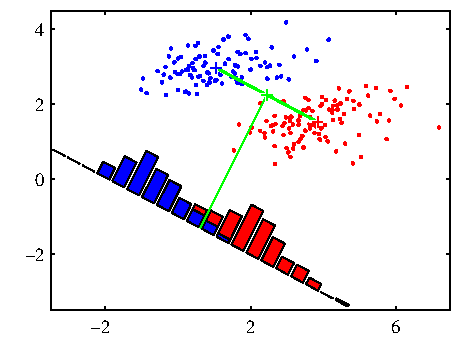
\includegraphics[width=1.2\textwidth]{Figure46a.pdf}

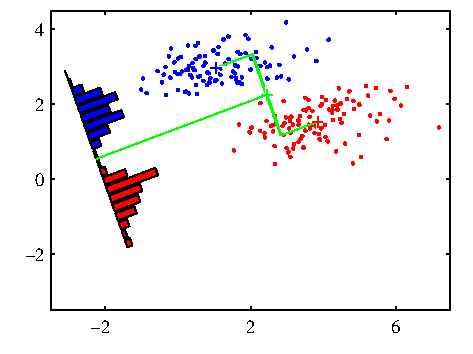
\includegraphics[width=1.2\textwidth]{Figure46b.pdf}

~\\
\tiny Bishop PRML Figure 4.6
\end{column}
\begin{column}{7.5cm}
\begin{itemize}
\item $\mathbf{m_+}= \frac{1}{N_+}\sum_{n \in C_+} x_n$ \hspace{.5cm} $\mathbf{m_{-}}= \frac{1}{N_-}\sum_{n \in C_{-}} x_n$ 
\item \pause Maximize projection-distance of class means 
[projected mean/variance: on board]
$\omega_{simple} \propto \mathbf{m}_+-\mathbf{m}_-$ 
\item \pause Maximizing distance between means ignores that the projected variances might also be big. 
\item \pause Fix:  Maximize the ratio of between-class variance to within-class variance ('signal to noise'). Fisher criterion
\begin{align}
J_\omega = 2\frac{(m_+-m_-)^2}{s_+^2+s_-^2}
\end{align}
[Details and solution: on board]
%\item 
\pause 
$\omega_{lda}= \Sigma_w^{-1} (\mathbf{m}_+-\mathbf{m}_-)$
\end{itemize}
\end{column}
\end{columns}

}
%http://users.informatik.uni-halle.de/~hinnebur/Lehre/BN_seminar_web/bn_05_ag.pdf


\frame{\frametitle{Aside: The multivariate Gaussian} 
\begin{itemize}
\item Probability density function of $D$ dimensional Gaussian with mean $\mu$ an covariance $\Sigma$: \begin{align}p(x| \mu, \Sigma)&= (2\pi)^{-D/2}|\Sigma|^{-1/2} \exp \left(-\frac{1}{2} (x-\mu)^\top \Sigma^{-1} (x-\mu) \right) \\
 \end{align}
\item \pause Maximum likelihood estimation of parameters: \begin{align}
\hat\mu= &\frac{1}{N}\sum_n x_n\mbox{~~(empirical mean)}\\ 
\hat \Sigma= &\frac{1}{N} \sum_n x_n x_n^\top- \hat\mu \hat \mu^\top\mbox{~~(empirical covariance)} 
 \end{align}
\end{itemize}
\begin{center}
\pause
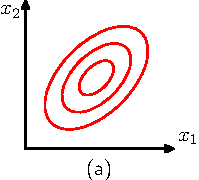
\includegraphics[width=.25\textwidth]{Figure28a.pdf}
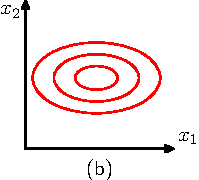
\includegraphics[width=.25\textwidth]{Figure28b.pdf}
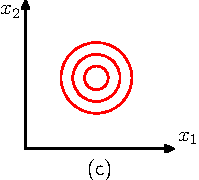
\includegraphics[width=.25\textwidth]{Figure28c.pdf}
\end{center}
~\\
\tiny Bishop PRML Figure 2.8
}

\frame[shrink=5]{\frametitle{A (super brief) primer on covariance matrices. (more details/intuition in second half of course?)} 
%\begin{columns}
%\begin{column}{4.5cm}

%\end{column}
\begin{center}
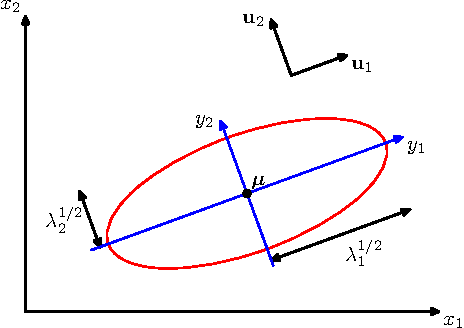
\includegraphics[width=.45\textwidth]{Figure27.pdf}
\\
\tiny Bishop PRML Figure 2.7
%\end{column}
\end{center}
%\begin{column}{8cm}
\begin{itemize}
\item \pause Covariance matrices are symmetric.
\item \pause Diagonal entries: variances along coordinate-axes
\item \pause Eigenvectors: principal axes of ellipsoid
\item Eigenvalues:  variances along eigen-vectors
\item Eigenvector with maximal/minimal eigen-value: Direction of maximal/minimal variance 
\item \pause Covariance matrices are `positive definite', i.e. all their eigenvalues are non-negative.
\item \pause Most of this can be derived from $a^\top \mbox{Cov}(X) a= \mbox{Var}(a^\top X)$
\end{itemize}
%\end{column}
%\end{columns}


}


\section{A generative model: Class-conditional Gaussians}
\frame{\frametitle{A tale of two Gaussian: We can use a probablistic model of the data for classification} 
\begin{center}
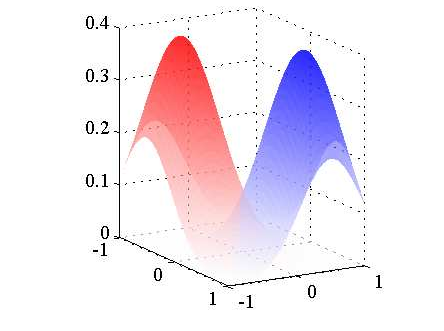
\includegraphics[width=.35\textwidth]{Figure410a.pdf}
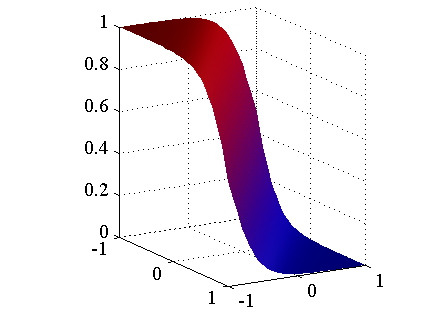
\includegraphics[width=.35\textwidth]{Figure410b.pdf}
\end{center}

\begin{itemize}
\item Suppose that each of the two classes is modelled by a Gaussian: $x | x \in C_+ \sim \mathcal{N}\left(\mu_+, \Sigma_+\right)$, $x | x \in C_- \sim \mathcal{N}\left(\mu_-, \Sigma_-\right)$, 
\item ~[On board] Calculation of posterior class probabilities and decision criterion
\item \pause If we assume $\Sigma_+=\Sigma_-$, we get $\omega_{gauss} \propto \Sigma_+^{-1} (\mathbf{m}_+-\mathbf{m}_-)$
\item Note: We take the $t_n$ as given and built a model of $x_n | t_n$, contrast with linear regression, where we took $x_n$ as given and modelled $t_n |x_n$.
\end{itemize}
\tiny Bishop PRML Figure 4.10
}

\frame{\frametitle{This approach directly generalizes to classification with unequal covariances and multi-class classification.}
\begin{center}
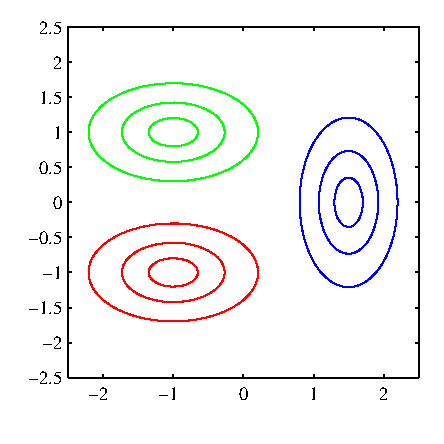
\includegraphics[width=.35\textwidth]{Figure411a.pdf}
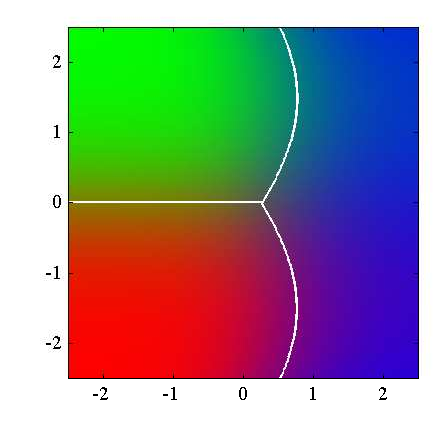
\includegraphics[width=.35\textwidth]{Figure411b.pdf}
\end{center}
\begin{itemize}
\item Quadratic discriminant analysis: $\Sigma_+ \neq \Sigma_o$, decisison boundary is of form $y(\xx) = \xx^\top A \xx+\omega^\top \xx +\omega_o$
\item Multi-class: Assign each data-point to class with highest posterior probability (or calculate best assignment from cost-function). 
\end{itemize}
\tiny Bishop PRML Figure 4.10
}

\frame{\frametitle{A simple nonlinear classifier can be constructed from kernel density estimates of the probability densities.}

\begin{columns}
\begin{column}{4cm}

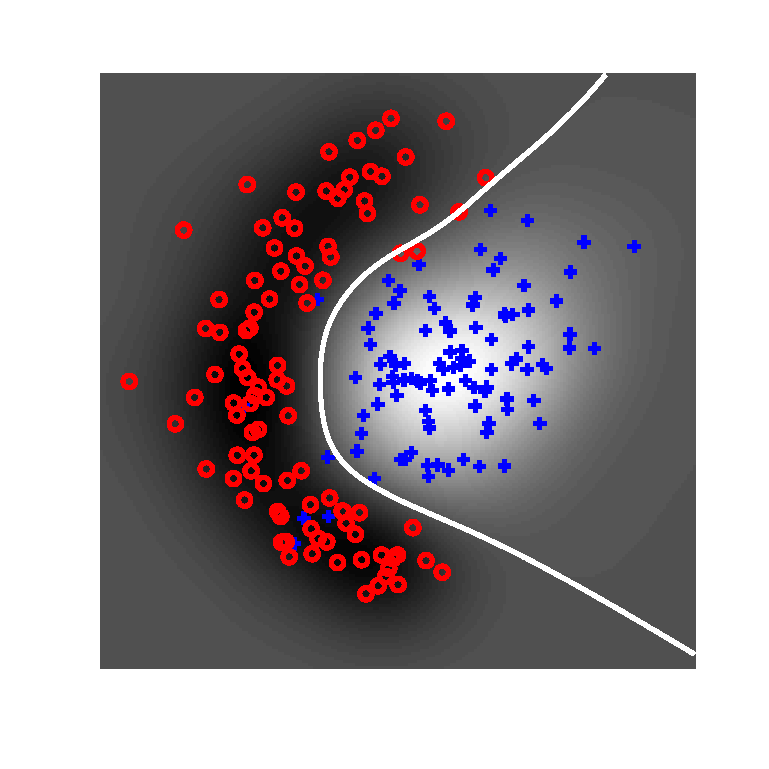
\includegraphics[width=\textwidth]{NonLinClassification.pdf}
\end{column}
\begin{column}{7cm}
\begin{itemize}
\item Idea: Once we have an estimate of the class-conditional densities $P(x| t=\pm 1)$, we can construct a rule from $d(x)=P(x| t=+ 1)-P(x| t=- 1)$.
\item \pause Use \alert{kernel density estimation} to estimate  $P(x| t=\pm 1)$, i.e. place a `Gaussian bump' on each data-point:
\begin{align}
P(x| t=1) =\frac{1}{Z}\sum_{n_+} \exp\left( \frac{x-x_n}{\sigma}\right)^2
\end{align}
\end{itemize}
\end{column}
\end{columns}
\pause
This leads to a classifier of the form
\begin{align}
d(x)= \sum_{n} \alpha  t_n \exp\left( \frac{x-x_n}{\sigma}\right)^2
\end{align}
\pause
\alert{Support vector machine with radial basis functions} has decision rule \begin{align}
d(x)=\sum_{n}  \alpha_n \exp\left( \frac{x-x_n}{\sigma}\right)^2
\end{align}
}




\frame{\frametitle{Summary: One for the price of three.} 
\begin{itemize}
\item Today, you learned about three different algorithms for binary classification with linear decision rules. 
\item \pause One was based on a hack, the second one on a plausible (but ad-hoc) criterion, and the third one an a probababilistic model of the data.
\item \pause All three algorithms are equivalent.
\item \pause We showed that the Fisher discriminant and the probabilistic model based on two Gaussians have the same  decision criterion. In fact, it can be shown that linear regression has the same weights (Bishop 4.1.5)
%\item \pause The moral: Great motivations are great, but the actual algorithm matters, and it is important to check connections with other algorithms.
\item The third motivation had immediate extensions to nonlinear algorithms and multi-class classification, and posterior probabilities.
\item \pause Next week, we will learn an algorithm which actually is different, and usually better than the ones discussed today.
\end{itemize}
}



\end{document}



